\documentclass[tikz,border=8pt]{standalone}
% Shared look for every TikZ diagram. Load with \input{../../tools/tikz-style.tex}
\usepackage[T1]{fontenc}
\usepackage{lmodern}
\renewcommand{\sfdefault}{lmr}  % diagrams use the same serif as the text
\usetikzlibrary{arrows.meta, positioning, shapes.geometric, calc, fit, backgrounds}
\definecolor{cblue}{HTML}{4C78A8}
\definecolor{corange}{HTML}{F58518}
\definecolor{cgreen}{HTML}{54A24B}
\definecolor{cred}{HTML}{E45756}
\definecolor{cpurple}{HTML}{B279A2}
\definecolor{cgrey}{HTML}{6B6B6B}
\tikzset{
  every picture/.style={font=\sffamily, line width=1.2pt},
  box/.style={draw=#1, fill=#1!12, rounded corners=4pt, align=center, inner sep=7pt, minimum height=1.1cm},
  box/.default=cgrey,
  arrow/.style={-{Stealth[length=3mm]}, draw=cgrey, line width=1.4pt},
  title/.style={font=\sffamily\bfseries\Large},
  note/.style={font=\sffamily\small, text=cgrey, align=center},
}
\AtBeginDocument{\hyphenpenalty=10000 \exhyphenpenalty=10000}

\begin{document}
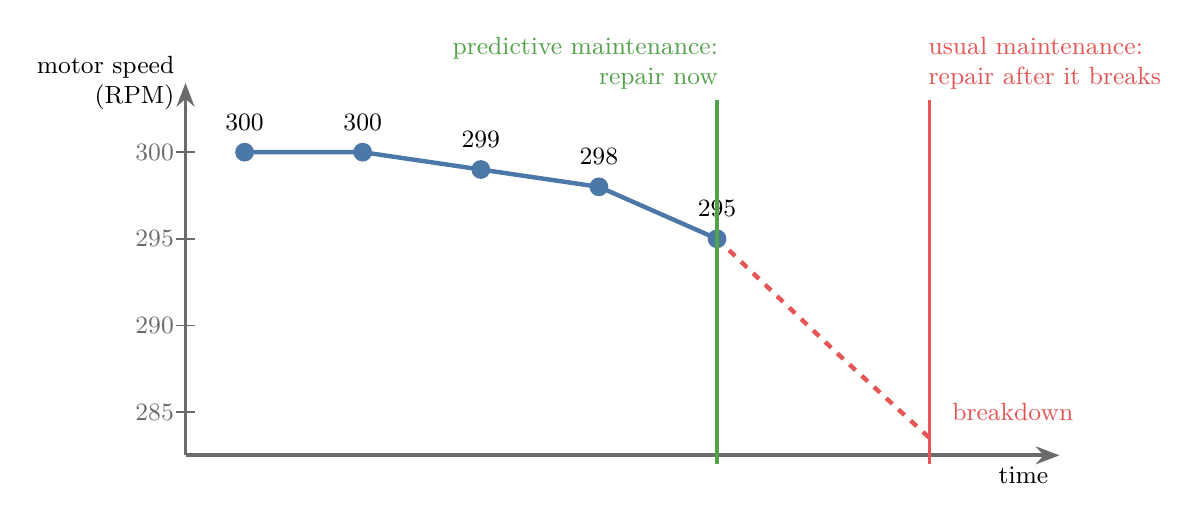
\begin{tikzpicture}[x=1.5cm, y=0.55cm]
  % axes
  \draw[arrow] (0,0) -- (7.4,0) node[below left, font=\small] {time};
  \draw[arrow] (0,0) -- (0,8.6) node[left, font=\small, align=right] {motor speed\\(RPM)};
  \foreach \v/\l in {1/285, 3/290, 5/295, 7/300} \draw[cgrey, line width=0.6pt] (-0.08,\v) -- (0.08,\v) node[left=4pt, font=\small] {\l};
  % readings: 300, 300, 299, 298, 295, then failure
  \draw[cblue, line width=1.6pt] (0.5,7) -- (1.5,7) -- (2.5,6.6) -- (3.5,6.2) -- (4.5,5);
  \draw[cred, dashed, line width=1.6pt] (4.5,5) -- (5.5,2.4) -- (6.3,0.4);
  \foreach \x/\y/\l in {0.5/7/300, 1.5/7/300, 2.5/6.6/299, 3.5/6.2/298, 4.5/5/295}
    \node[fill=cblue, circle, inner sep=2.4pt, label={[font=\small]above:\l}] at (\x,\y) {};
  \node[note, text=cred, anchor=west] at (6.4,1.0) {breakdown};
  % markers
  \draw[cgreen, line width=1.2pt] (4.5,-0.2) -- (4.5,8.2);
  \node[note, text=cgreen, anchor=south east, align=right] at (4.6,8.2) {predictive maintenance:\\repair now};
  \draw[cred, line width=1.2pt] (6.3,-0.2) -- (6.3,8.2);
  \node[note, text=cred, anchor=south west, align=left] at (6.2,8.2) {usual maintenance:\\repair after it breaks};
\end{tikzpicture}
\end{document}
